
\newcommand{\md}{\mathrm{d}}

\section{Gravitational Waves}

\subsection{Serendipitous Detections of Kilonovae}
\textit{Authors: Christian N. Setzer\footnote{christian.setzer@fysik.su.se}, Rahul Biswas, Hiranya V. Peiris}\newline
\newline
Part of the power of LSST is to detect many transients on a nightly basis \citep{LSSTScienceCollaboration2009}. This includes detections of rare transients, such as kilonovae (KNe). With the event GW170817, we now know that gravitational waves can be accompanied by an electromagnetic signal as was long theorized since we can get cosmological constraints even from a single event, ($H_0 = 70.0^{+12.0}_{-8.0} \mathrm{km\,s^{-1}\,Mpc^{-1}}$) \citep{Abbott2017}. This is predicated on the assumption that we will detect the counterpart gravitational wave signal. A question that could be asked is, what are we able to do with detections of kilonovae if we only obtain the electromagnetic counterpart? Could this be used to enhance the detectability of the
gravitational wave signal, by giving a prior on the signal? Before investigating these questions, however, it is useful to understand how many of these objects we would be able to detect. Due to the short lifetime and lower luminosity of these events, in comparison to more abundant and bright transients like supernovae, we expect that the numbers we are able to detect to be sensitive to many features of the cadence.\par

\subsubsection{Background}
With the event of last summer being the only known observation of a kilonova it is a good starting place to assume the time-series spectral energy distribution (SED) will be the same as this event. To characterize that event we use the time-series SED, provided by the Dark Energy Survey (DES), that was used in the analysis of \citep{Scolnic2017a}. This model uses multi-band photometry to calibrate a spectral time-series to observations, the photometry comes from \citep{Soares-Santos2017, Cowperthwaite2017}. However, it would also be naive to assume that this event represents the electromagnetic properties of all events of this type. Thus we would like to test a model that is physically motivated that spans a parameter space that describes the population. We have chosen a semi-analytic model for the SED evolution of KNe by \citep{Rosswog2018}. The semi-analytic model, while one-dimensional, uses a sophisticated radiation transport treatment building on the works of \citep{Wollaeger2017, Pinto2000}. This model uses three parameters, the gray opacity ($\kappa$), the median ejecta mass ($\mathrm{m_{ej}}$), and the median ejecta velocity ($\mathrm{v_{ej}}$) to generate the time-series SED evolution for a KN event. \par
\begin{table}[h!]
  \centering
  \begin{tabular}{c|c|c}
    Rosswog Model Parameter & Range & Units \\
    \hline
    $\kappa$ & $\mathrm{binomial}[1, 10]$ & $\mathrm{cm^2 g^{-1}}$ \\
    \hline
    $\mathrm{m_{ej}}$ & $[0.01, 0.2]$ & $\mathrm{M_{\bigodot}}$ \\
    \hline
    $\mathrm{v_{ej}}$ & $[0.01, \, 0.5 (\mathrm{m_{ej}}/0.01)^{-\mathrm{log}_{20}(2)}]$ & c
  \end{tabular}
  \caption{The space of parameters that describe the population of KNe in the Rosswog semi-analytic model. This range comes from the previous exploration of the parameter space in \citep{Rosswog2016a}.}
  \label{tab: ross_params}
\end{table}

The space spanned by these parameters is shown in Table \ref{tab: ross_params}, also see Fig. \ref{fig: ross_params}. A note on the bounds, for $\mathrm{v_{ej}}$, this bound was set based on the condition that the total energy of the event stayed under $10^{52}\, \mathrm{ergs}$ as given by the bounds of Rosswog et. al in their exploration of this parameter space with numerical hydrodynamics simualtions \citep{Rosswog2016a}. The relation is a first approximation to the line of constant energy shown in Fig. 4 of their paper \citep{Rosswog2016a}. The bound on the gray opacity, being a binomial distribution, was used due to the high uncertainty in this parameter for KNe \citep{Kasen2013} and this being a standard assumption in the numerical simulation community \citep{Rosswog2018}.\par

\begin{figure}[t!]
  \centering
  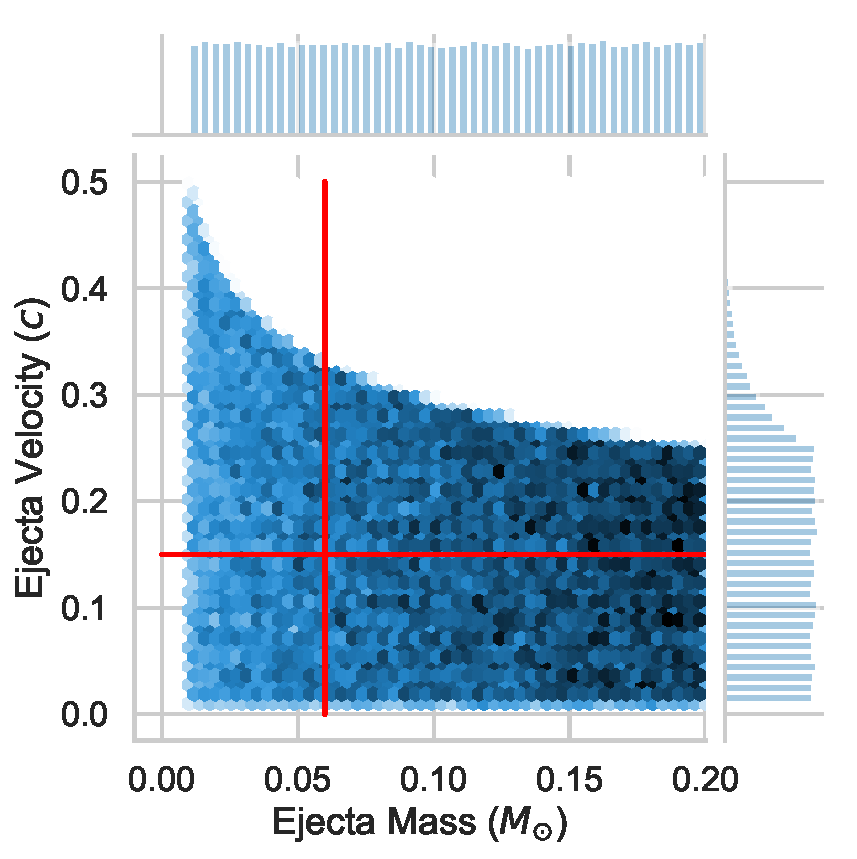
\includegraphics[scale=0.55]{figures/Rosswog_parameter_dist}
  \caption{The parameter space of the two continuously varying parameters which characterize the population of KNe of the Rosswog model. The intersection of the red lines shows where, as determined by \citep{Rosswog2018}, the event GW170817 falls within the parameter space for a best fit to the infrared photometric light curves.}\label{fig: ross_params}
\end{figure}

To simulate observations of KNe we begin with the number of transient events per co-moving volume per event rest-frame time, which we call the co-moving event rate density:

\begin{equation}\label{eqn:erd}
   \Gamma_{\mathrm{co}} =\frac{\md N_{\mathrm{total}}}{\md V_{\mathrm{co}}\md t_{\mathrm{rest}}}.
\end{equation}\par

This rate, $\Gamma_{\mathrm{co}}$, is often assumed to be constant as we do here. We now wish to compute the redshift distribution of such events in the observer's frame. We can now define the distribution of events in redshift space, $n_{\mathrm{events}}$, and the cumulative number of events, $N_{\mathrm{total}}$, observed out to some redshift. These two quantities are related by,

\begin{equation}\label{eqn:total_dist}
N_{\mathrm{total}}(z) = \int_0^{z} n_{\mathrm{events}}(z) \md z.
\end{equation}\par
Further, from Eq. \ref{eqn:erd} we obtain,
\begin{equation}
N_{\mathrm{ total}}(z) = \int_0^{T (z)} \int_0^{V_{\mathrm{co}}(z)}  \Gamma_{\mathrm{co}} \md V_{\mathrm{co}}(z)\md t_{\mathrm{rest}},
\end{equation}\par

where $T(z)$ is the total time elapsed in the rest frame at redshift $z$. This allows us to make the substitutions with cosmological quantities and obtain expressions for the redshift distribution. In terms of quantities directly relatable to known properties of the observations (observation time-interval, $\Delta T_{\mathrm{obs}}$, redshift, $z$, and the sky area, $\Delta \Omega_{\mathrm{obs}}$), we find the redshift distribution,\par

\begin{align}\label{eqn:reddist}
n_{\mathrm{events}}(z) = \, c^3  \frac{\Gamma_{\mathrm{co}}}{(1+z)H(z)} \left[\int^{z}_0 \frac{\md z'}{H(z')} \right]^2 \, \Delta T_{\mathrm{obs}} \Delta \Omega_{\mathrm{obs}}.
\end{align}\par

This concerns counts of events. The number of observed events then follows a Poisson distribution, where $k$ is the recorded counts, and the cumulative distribution function equal to,

\begin{equation}\label{eqn:invcum}
P(k;N_{\mathrm{total}}(z)) =e^{-N_{\mathrm{ total}}(z)} \sum_{i=0}^k \frac{N_{\mathrm{ total}}(z)^i}{i!}.
\end{equation}\par

We can now choose a maximum redshift, $z_{\mathrm{max}}$, and, computing $N_{\mathrm{ total}}$, obtain a realization of the observed events. As this is a discrete distribution, we must use an approximation of inverse of the cumulative probability distribution function \ref{eqn:invcum}. This is done by drawing from a uniform unit interval distribution, $u\in(0,1]$, which represents evaluations of the cumulative distribution function. Then, as we know the values of Eq. \ref{eqn:invcum}, we find the value of $k$ which gives the closest value to our draw, $u$, from the uniform distribution. This $k$ corresponds to the realization of the total number of events from the Poisson distribution, $N_{\mathrm{ total}}^{\mathrm{realization}}$. With this realization we can then build a realization of the redshift distribution.\par

Given the cumulative redshift distribution of events, $N_{\mathrm{total}}(z)$, we can scale this to the total number of events $N_{\mathrm{total}}(z_{\mathrm{max}})$. This is equivalently a cumulative probability distribution function of transient events as a function of redshift, $F(z) = N_{\mathrm{total}}(z)/ N_{\mathrm{total}}(z_{\mathrm{max}})$. Next, take draws from a uniform unit interval distribution, $u_i\in(0,1]$, where $i$ runs from $1$ to $N_{\mathrm{ total}}^{\mathrm{realization}}$. Then, using the inverse of the cumulative distribution function, map these draws from the uniform distribution to the redshifts which generate these values, $F^{-1}(u_i) \rightarrow z_i$. This produces a set of redshifts for all the transient events that happen within the observer frame represented by $\Delta \Omega_{\mathrm{obs}}$, $\Delta T_{\mathrm{obs}}$, and the redshift range, $z \in [0,z_{\mathrm{max}}]$, considered.\par

\subsubsection{Simulations}
With the number of events and their redshift distribution calculated, we then place the KNe uniformly in right ascension and declination within the declination band that covers the entire LSST sky footprint for a given cadence. Additionally, the time of explosion is chosen uniformly within the survey lifetime. Then, given either the empirical DES-GW model for the KNe or the Rosswog KNe model we generate a time-series SED for each event that is then redshifted, dimmed, and extincted according to the pairing of redshift, right ascension, and declination that it has been assigned. Each object is also assigned a peculiar velocity which doppler shifts the SED as well. A summary of all these parameter choices is in Table \ref{tab: sim_params}.\par

\begin{table}[h!]
\centering
\resizebox{\columnwidth}{!}{%
  \begin{tabular}{c|c|c}
  Simulation Parameter & Values & Note \\
  \hline
$z$ & $[0, 0.5]$ & $z_{\mathrm{max}}$ at Einstein Telescope Sensitivity \citep{Chen2017a}. \\
 \hline
$R_{\mathrm{KN}}$ & $1000 \mathrm{Gpc^{-3} \,yr^{-1}}$ & Rate used in \citep{Scolnic2017a}. \\
\hline
Dust Map & Per-bandfilter extinction & SFD \citep{Schlafly2011} \\
\hline
Peculiar Velocity & Gaussian($\mu = 0; \sigma = 300 \mathrm{km\, s^{-1}}$) & `Typical' values \citep{Davis2010}.
  \end{tabular}
}
 \caption{The space of parameters that describe the population of KNe in the Rosswog semianalytic model.}\label{tab: sim_params}
\end{table}

With this distribution in place, the cadence specified by an OpSim database is then applied as a filtering to make observations of each event. For a given transient, all pointings that overlap with the event's spatial location and lifetime are found, assuming a circular field-of-view geometry, and the instrument measured flux and other observational properties are computed. These observations then pass through a second stage of filtering given by the criteria for detection.\par

\subsubsection{Metric}
The metric we have chosen for evaluation of a cadence is the number of KNe that are detected given the simulations of observations given above. The criteria that we use to determine detections is that of \citep{Scolnic2017a}. These criteria are the following:
\begin{itemize}
  \item Two alerts separated by $\geq 30$ minutes.
  \item Observations in at least two filters with $\mathrm{SNR} \geq 5$.
  \item Observations with $\mathrm{SNR} \geq 5$ separated by maximum 25 days.
  \item At minimum one observation of location within 20 days before the first $\mathrm{SNR} \geq 5$ observation.
  \item At minimum one observation of location within 20 days after the last $\mathrm{SNR} \geq 5$ observation.
\end{itemize}

In this context an alert is an observation that has an observed signal-to-noise ratio greater than five after template subtraction. This is simulated using the per-filter efficiency vs. true signal-to-noise ratio response function. As this function is unknown for LSST prior to operation, we have used the set of functions that were found for the DES year-one analysis given their filter-set is quite similar to LSST [R. Kessler, private communication]. With this criteria the observations are filtered and the subset of transients which pass all conditions are then labeled as detections.\par
Given that these are the detection results for kilonovae using a single realization of the redshift distribution for each cadence, which are themselves a draw from a Poisson distribution as explained above, the uncertainty on these values, is the square root of the sample mean. For the case of one sample, this is the number of detections that are found per cadence, so the uncertainty on number of detections is the square root of the numbers of detections.\par
\begin{figure}[h!]
  \centering
  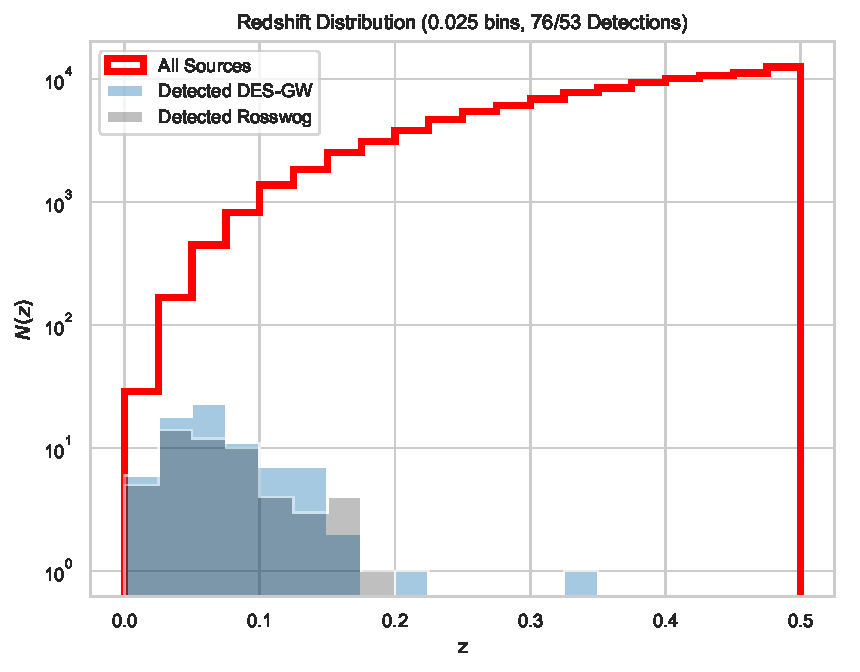
\includegraphics[scale=0.72]{figures/both_nz_base_kraken_2026}
  \caption{Example redshift distribution of detected KNe within the sample of all simulated KNe. This distribution is for the unofficial project baseline cadence \protect \textit{kraken 2026} for the DES-GW KNe SED model with an inlay of the results for the same cadence for the Rosswog model.}
  \label{fig:typical_nz}
\end{figure}
\subsubsection{Results}
The results, see Fig. \ref{fig:cadence_ranking} and \ref{fig:cadence_ranking_ddf}, are a simple ranking of the cadences for each KNe based on the number of detections metric. Immediately we conclude the DES-GW model, which is based on a single event, predicts a larger number of detections than the model of Rosswog, which describes a population of events. This is at least in part to the `blue flash' as described in many papers about the discovery, which is absent from most models of KNe \citep{Villar2017b}. Additionally, as was concluded in the paper by Scolnic et. al, the majority of our detections will come from the wide-fast-deep region of the survey as opposed to the deep-drilling-fields \citep{Scolnic2017a}. The typical redshift range of detected KNe, as shown in Fig. \ref{fig:typical_nz}, is between $0 \leq z \leq 0.2$, though some detections can extend out to $z \approx 0.3$. While this varies between cadences and models, this range is quite typical between all the cadences considered. The effect of changing KNe model, which can also be seen in Fig. \ref{fig:typical_nz} is that the numbers are slightly suppressed and the lack any high redshift outlier detections.\par
\begin{figure}[h!]
  \centering
  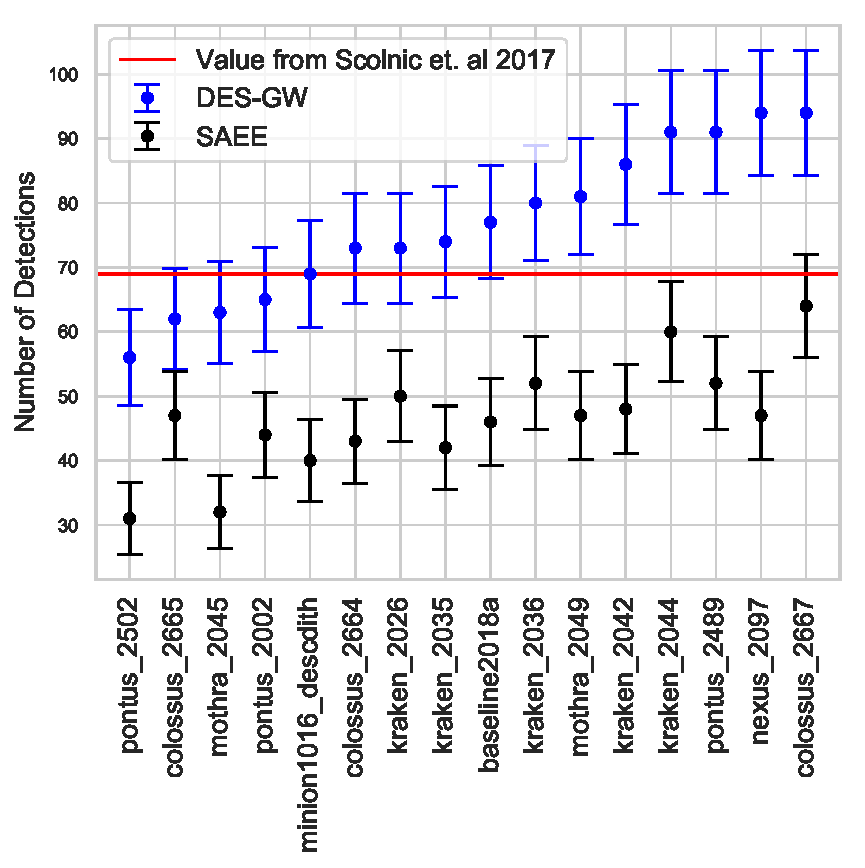
\includegraphics[scale=0.7]{figures/wfd_detection_counts_by_cadence}
  \caption{Ranking of cadence strategies for the WFD part of the survey for both KNe models, based entirely on the number of detections found in each cadence.}
  \label{fig:cadence_ranking}
\end{figure}

\begin{figure}[h!]
  \centering
  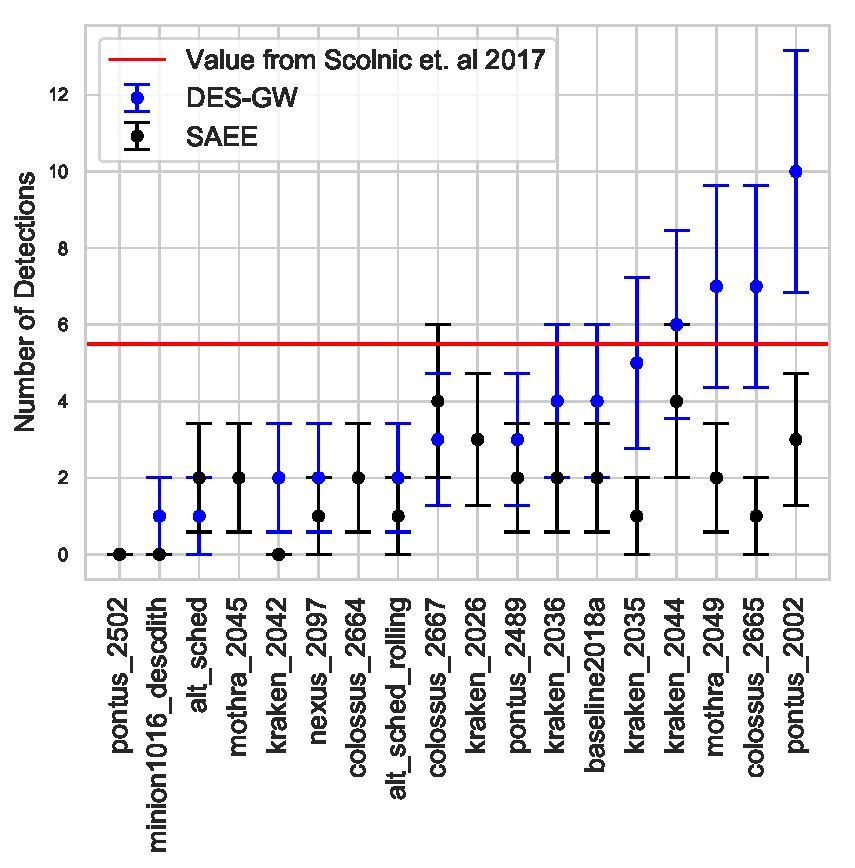
\includegraphics[scale=0.7]{figures/ddf_detection_counts_by_cadence}
  \caption{Same as the above figure but for the DDF.}
  \label{fig:cadence_ranking_ddf}
\end{figure}

\FloatBarrier
